\section{実験手法}
\subsection{スズ-Ge合金試料(β相)の作成}
試料作成は理化学研究所吉川氏の指導のもと、理化学研究所の設備を用いて行った。まず、高純度の粒状のスズと粒状のGe(\textcolor{red}{??\%})をエタノールで超音波洗浄にかけた。その後同じく洗浄したすり鉢で、Geをすりつぶし粉状にした。それらを以下に記述するように混合したあと電気炉(\textcolor{red}{??})やアーク炉(\textcolor{red}{??})またはヒートガンを用いた三種類の手法で溶融し、常温まで冷却した。

\subsubsection{封管試料の電気炉での加熱}
電気炉を用いた溶融法は温度履歴を管理できる点に強みがある。本実験ではGe濃度0.1 wt. \%(質量\%)、0.5 wt. \%、1 wt. \%の三通りについて、冷却速度をコントロールした試料を作成した。表\ref{tab:sample_prep_elec}に電気炉を用いた試料作成実験の諸元(Ge濃度、最高到達温度、冷却方法)を示す。
\begin{table}[!h]
    \begin{center}
  \begin{tabular}{c|cccccc}
    & 試料1 & 試料2 & 試料3 & 試料4 & 試料5 & 試料6 \\ \hline
    Ge濃度(wt. \%)  & 1 & 0.5 &  0.1 & 50 & 1 & 1\\
   最高到達温度(℃)  & 1050 & 1050 &  1050 & 400& 400 & 1050 \\
    冷却方法 & 水クエンチ & 水クエンチ& 水クエンチ& 水クエンチ& 水クエンチ &徐冷(48時間)   \\
  \end{tabular}
  \caption{試料作成の諸元}
  \label{tab:sample_prep_elec}
    \end{center}
\end{table}

試料1、2、3はそれぞれ、スズとGeがお互いに溶けあい均一な液相となったあと急冷した試料である。まず洗浄した粒状のスズ2gを電子天秤を用いて計量し、石英管に入れたあと、Geが1 wt. \%(試料1)または0.5 wt. \%(試料2)または0.1 wt. \%(試料3)となるようGe粉末を石英管に入れた。Ge粉末を石英管に入れる際は、計量したGe粉末を正確に混合できるようアルミ箔を細長く切って折りガイドにし、静電気で石英管内面にくっつかないようにした。その後、石英管を真空ポンプで減圧し、石英管の中ほどを水素バーナーで加熱し封管した。図\ref{fig:GeSn_phase}のSn-Ge合金試料の相図によると、Sn-Ge合金試料はその組成によらず1000℃を越えると完全に溶解する。試料1,2,3を封管された石英管ごと電気炉を用いて加熱し、1050℃に達したあとよくふって混合して、石英管のまま水の中に浸して急冷した(水クエンチ)。

試料6は、スズとGeがお互いに溶けあい均一な液相となったあと徐冷した試料である。試料1,2,3と同様に、Geが1wt.\%濃度となるよう混合し、電気炉を用いて1050℃まで加熱したあと、48時間かけて室温まで徐冷した。

試料4は、スズとGeがお互いに溶けあわない不均一な状態で急冷した試料である。試料1,2,3,6と同様に混合したあと、スズ単体の融点とGe単体の融点の間の400℃まで加熱し、石英管を水の中に浸し急冷した。スズとGeは室温で分離しているため、スズ液相中にGeが溶け込むには時間がかかる。それをあえて待たずに水クエンチした。

試料5ではスズとGeの界面の状態を観察するために、粒状スズと粉末Geを質量比1:1で1gずつ混合した。それらをスズ単体の融点とGe単体の融点の間の400℃まで加熱したあと、急冷した試料である。こちらも試料4と同様に、不均一な状態で水クエンチした。

\subsubsection{アーク炉での加熱}
アーク炉内では温度分布が一様でなく温度履歴を管理できないが、簡便な手法である。本実験ではGe濃度0.1 wt. \%(質量\%)、1 wt. \%の二通りについて、アーク炉の出力を変化させた。表\ref{tab:sample_prep_arc}にアーク炉を用いた加熱法の諸元(Ge濃度、アーク炉の出力、冷却法)を示す。
\begin{table}[!h]
    \begin{center}
  \begin{tabular}{c|cccc}
    & 試料7 & 試料8 & 試料9 & 試料10 \\ \hline
    Ge濃度(wt. \%)  & 1 & 0.1 &  1 & 0.1  \\
   アーク炉の出力  & 最大& 最大&  半分以下 & 半分以下\\
    冷却方法 & 急冷 & 急冷& 急冷& 急冷 \\
  \end{tabular}
  \caption{アーク炉を用いた試料作成の諸元}
  \label{tab:sample_prep_arc}
    \end{center}
\end{table}

試料7、8は、試料1、2、3と同様にスズとGeがお互いに溶けあったあと急冷することを目指した試料である。一方、アーク炉のサンプルステージは熱伝導のよい銅でできており絶えず水で冷却しているので、石英管中の試料1,2,3よりも速い冷却速度が期待できる(\textcolor{red}{?})。Geが1 wt. \%(試料7)と0.1 wt. \%(試料8)となるように粒状スズと粉末Geを混合したあと、サンプルステージに置き、電極を近づけアーク電流を最大出力で流したあと、電流を切った。

試料9、10は、アーク炉の出力を試料7、8の半分以下とした。Ge濃度が1 wt. \%(試料10)と0.1 wt. \%(試料8)となるよう同様に混合したあとサンプルステージに置き、電流を最大出力の半分以下で流したあと、電流を切った。試料4と同様に、スズとGeがお互いに溶けあわない不均一な状態で急冷された。

\subsubsection{ヒートガンでの加熱}
ヒートガンは小型の簡単な熱源であるため400℃以上の高温には到達できないが、アーク炉に比べてさらに簡便である。ヒートガンを用いた簡便な試料作成法が確立できれば、気軽に様々な場所で試料作成できて作成条件の最適化に向いている。本実験ではGe濃度0.1 wt. \%(質量\%)、0.1 wt. \%、0 wt. \%の三通りについて、試料を作成した。表\ref{tab:sample_prep_heatgun}にヒートガンを用いて加熱した際の諸元(Ge濃度、冷却法)を示す。
\begin{table}[!h]
    \begin{center}
  \begin{tabular}{c|cccc}
    & 試料11 & 試料12 & 試料13 \\ \hline
    Ge濃度(wt. \%)  & 1 & 0.1 &  0  \\
    冷却方法 & 放冷 & 放冷 & 放冷 \\
  \end{tabular}
  \caption{ヒートガンを用いた試料作成の諸元}
  \label{tab:sample_prep_heatgun}
    \end{center}
\end{table}

試料11、12、13は、試料1、2、3、6と同様に粒状スズと粉末Geを石英管に入れた。その石英管を真空ポンプで減圧した状態でヒートガンを押し当てて加熱し、スズが液体となったら加熱をやめ空気中で放冷した。

以上の手法により溶融した11通りの試料(as grown試料)のうち、一部の試料4、5、9、11などに関してはGeが表面に塊のまま分布しており、空間的にGe濃度が不均一だった。

Ge濃度が一様な残りの試料は全て金属的な光沢を持っており柔らかく延性をもっていることから、金属である。実際、\ref{sec:Xray_experiment}章と\ref{sec:Xray_results}章に記述するX線回折実験により、特に試料1、2、3、6は金属のβスズ構造であることを確かめた。

\subsection{αスズ試料への変換}
本研究の目的を達成するためにはパルスを用いてβスズをαスズに変換するだけではなく、αスズをβスズに変換しなければならない。また序論で述べたようにαスズをβスズに変換する方が逆の過程に比べ、かかる時間が短く簡便である。したがって筆者はいずれβスズに変換することを目的として、一部のAs grownのβスズ試料を(パルスを用いない準静的な過程により)αスズに相転移させた。

βスズからαスズへの相転移は230Kから260Kでおきる\cite{Matvienko,Ogino,Cornelius}。家庭用冷蔵庫の冷凍室はその温度がJIS規格により定められており-18℃(255K)以下であるため、βスズをαスズに相転移させる際の保管庫として利用できる。筆者はβスズ試料をダイアモンドカッターを用いてスライスして測定に適した形状に加工したのち、冷凍庫に保持しβスズからαスズへの相転移を観察した。またその際の相転移にかかった時間をおおまかに記録した。

さらに試料1に関してはαスズへの変換に長い時間がかかったので、表面加工やGeを押し付けるなどの工夫を行い、相転移にかかる時間を記録した。試料はα-β相転移する際に27\%程度の体積変化を伴うため、試料の核生成は試料の内部より表面から始まりやすく、また表面よりもエッジから始まりやすい\cite{Cornelius}。またαスズに変換するためにαスズそのものや、GeやSiのようなαスズと同じダイアモンド構造などをβスズに押し付けると、その部分から相転移が始まりやすいことが知られている\cite{Cornelius}。筆者は試料1に対して核生成を促進するためにカッターナイフで傷をつけたり、ニッパーで切り込みを入れたり、試料2のαスズを押し付けるなどの工夫を行った。

\subsection{試料のX線回折による評価}
\label{sec:Xray_experiment}
As grownのβスズ試料と家庭用冷凍庫に保持しαスズに転移した試料に関して、それぞれX線回折実験を行った。測定には理化学研究所のX線回折装置(Rigaku\textcolor{red}{??\%})を用いた。

X線源には熱電子が銅ターゲットで制動放射される際に出るCuKα線(特性X線)を用い、測定は$\rm 2\theta/\theta$配置で行った。図に$\rm 2\theta/\theta$配置の入射光と試料と回折光の位置関係の模式図を示す。X線は試料に入射角$\rm \theta$で入射し、Braggの回折条件$2d\:sin\theta=\lambda$を満たすとき、出射角$\rm \theta$で回折する。ただし$d$は基板に平行な格子面間隔であり、$\lambda$は特性X線の波長である。したがって角$2\theta$は回折角度に対応する。$\rm 2\theta/\theta$配置ではX線検出感度を高くできる。
\begin{figure}[!h]
    \begin{center}
   \includegraphics[width=0.8\hsize]{experiment/schematics_Xray.eps}
  \end{center}
  \caption{X線回折測定($\rm 2\theta/\theta$配置)の模式図}
  \label{fig:schematics_Xray}
\end{figure}

試料の結晶構造を精度よく同定するためには、試料がX線源と検出器の光軸が交わる領域に存在し、高さ方向に基板から出っ張っりすぎていない必要がある。

%\subsection{スズ-Ge合金試料(β相とα相)のEdX}

\subsection{α-β転移温度の測定}
スズはα-β相転移の前後で抵抗が大きく変化する。試料2、3、6、7について加熱しながら抵抗測定を行い、相転移温度を見積もった。試抵抗測定を横磁場クライオスタット(Oxford \textcolor{red}{??})を用いて、通常の4端子法により行った。

\subsection{電流パルスを用いたα相からβ相への変換}
まず、試料に電流パルスを印加してオーム発熱により加熱し、α相からβ相に相転移を起こすことを目標とした。またパルス印加中の抵抗測定も行い、抵抗変化から相転移を確認した。その際用いた電気回路の模式図を図\ref{fig:schematics_pulse}に示す。ソースメータ(Keithley 2400)から出力されたパルス電圧は、パワーアンプ(NF Corp. 4502)で100倍に増幅されたあと、光学クライオスタット中の試料とロード抵抗の直列接続に印加される。回路に流れる電流の時間変化は、$\rm 5.4\Omega$のロード抵抗の電圧降下をデータロガー(MC DT8824)で読み取り計算した(Ch2)。また試料の電圧降下もデータロガー(MC DT8824)で読み取り計算した(Ch1)

電流パルスにより相転移温度まで試料の温度を上げて、相転移前後で端子がくっついた状態を維持するためには、いくつかの技術的な工夫が欠かせない。まず筆者は試料を通常の四端子測定と同様に銀ペーストで端子付けして25Kに保持し、電流パルスを印加したところ、相転移温度までの温度上昇に少なくとも1.3A程度以上の電流が必要だった。したがって銀ペーストによる試料への端子づけではオーム発熱が十分でない。またそれ以上の電流を流すと直径$\rm 25 \mu m$の金線が焼き切れた。したがって電流端子に繋ぐ金線は$\rm 25 \mu m$では細いので、取り替える必要がある。また銀ペーストやカーボンペースト、金線を用いた端子付けに関する注意事項に関しては付録\ref{sec:4terminal}に詳述する。

筆者は試行錯誤の結果、図\ref{fig:schematics_sample}のような構成をとって電流パルスを印加するセットアップを見出した。前述したように、カーボンペーストは発熱に十分に高い抵抗が実現できる一方で機械的な強度が低く、銀ペーストは強度が高い一方で抵抗が小さい。そこでカーボンペーストで金線をコーティングした後、銀ペーストでサンプルにしっかりと接続した。この手法は十分に高い抵抗を実現しながら、機械的な強度も確保できると筆者は考える。さらに導線を高抵抗率のカーボンペーストを低抵抗率の銀ペーストで覆うことで、試料と金線の間に電流のパスが集中せず、比較的一様な加熱が可能となった。また電流端子につなぐ金線は1A程度以下の電流で焼き切れないように直径$\rm 50 \mu m$のものとした。一方、電圧端子をつなぐ線には大電流が流れないため、柔らかく熱伝導の高すぎないものとしたかった。そこで直径$\rm 25 \mu m$の金線とした。

また試料にパルス印加するのに前後して、抵抗の温度依存性を測定した。抵抗の温度依存性を測定するときの電気回路の模式図を図\ref{fig:schematics_lockin}に示す。ロックインアンプ(Stanford Research SR830)から出力した105Hzの交流電圧は、光学クライオスタット中の試料とロード抵抗の直列接続に印加される。回路に流れる電流は$\rm 150\Omega$のロード抵抗の電圧降下をマルチメータ(Keithley 2001)で読み取り算出した。試料の電圧端子間の電圧効果はトランス増幅器(Stanford Research SR554)で100倍に増幅したあと、ロックインアンプの入力端子に入力した。回路に流す電流値は、パルス電流で温度上昇しなかった値より十分小さくとった。また試料の複素インピーダンスの虚部(位相進み/遅れ)成分は実部の1/100程度以下だったので無視して、実部のみを抵抗とした。
\begin{figure}[!h]
 \begin{minipage}{\hsize}
    \begin{center}
   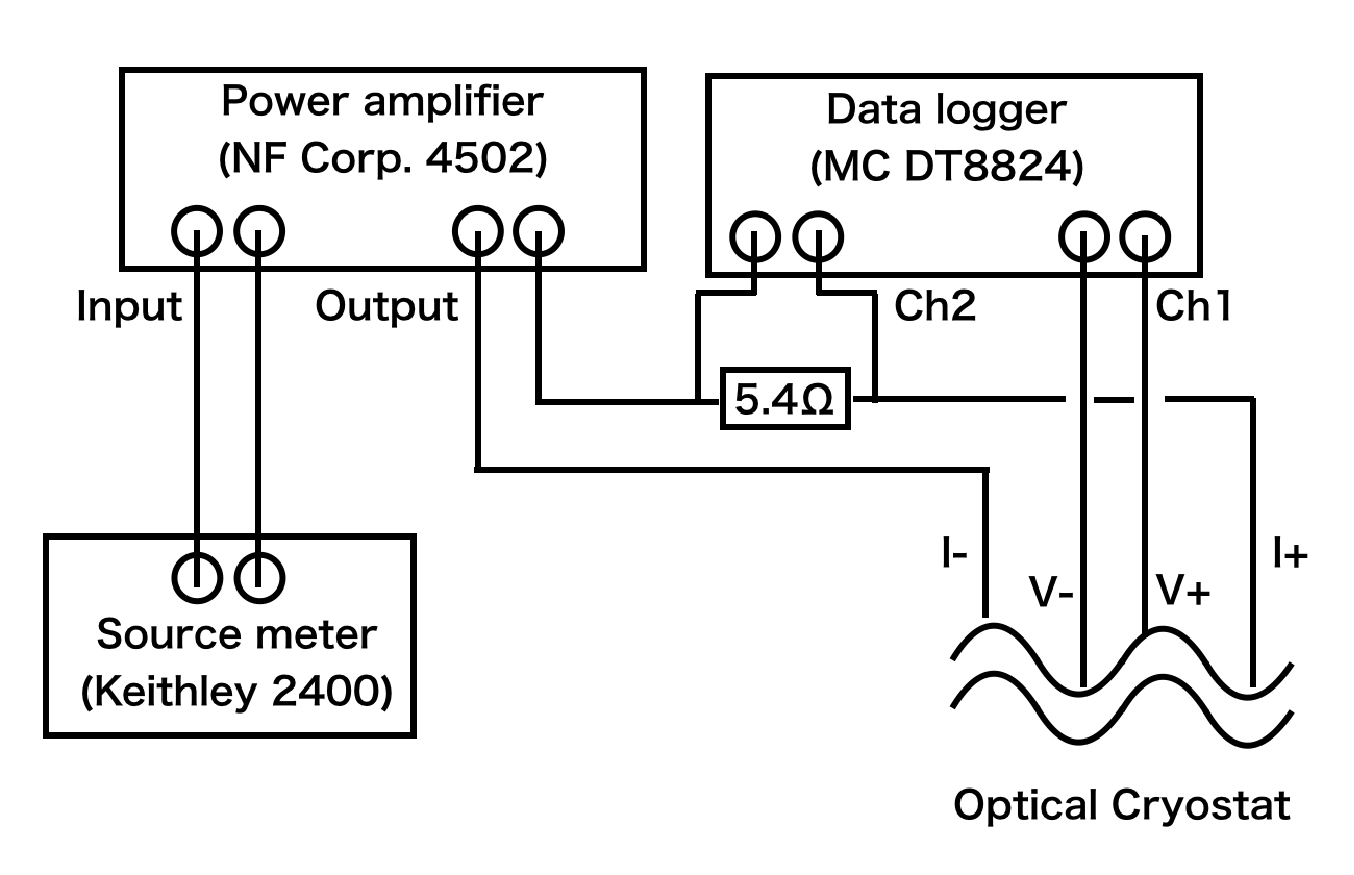
\includegraphics[width=0.7\hsize]{experiment/schematics_pulse.eps}
  \end{center}
  \caption{}
  \label{fig:schematics_pulse}
 \end{minipage}
 \begin{minipage}{\hsize}
     \begin{center}
   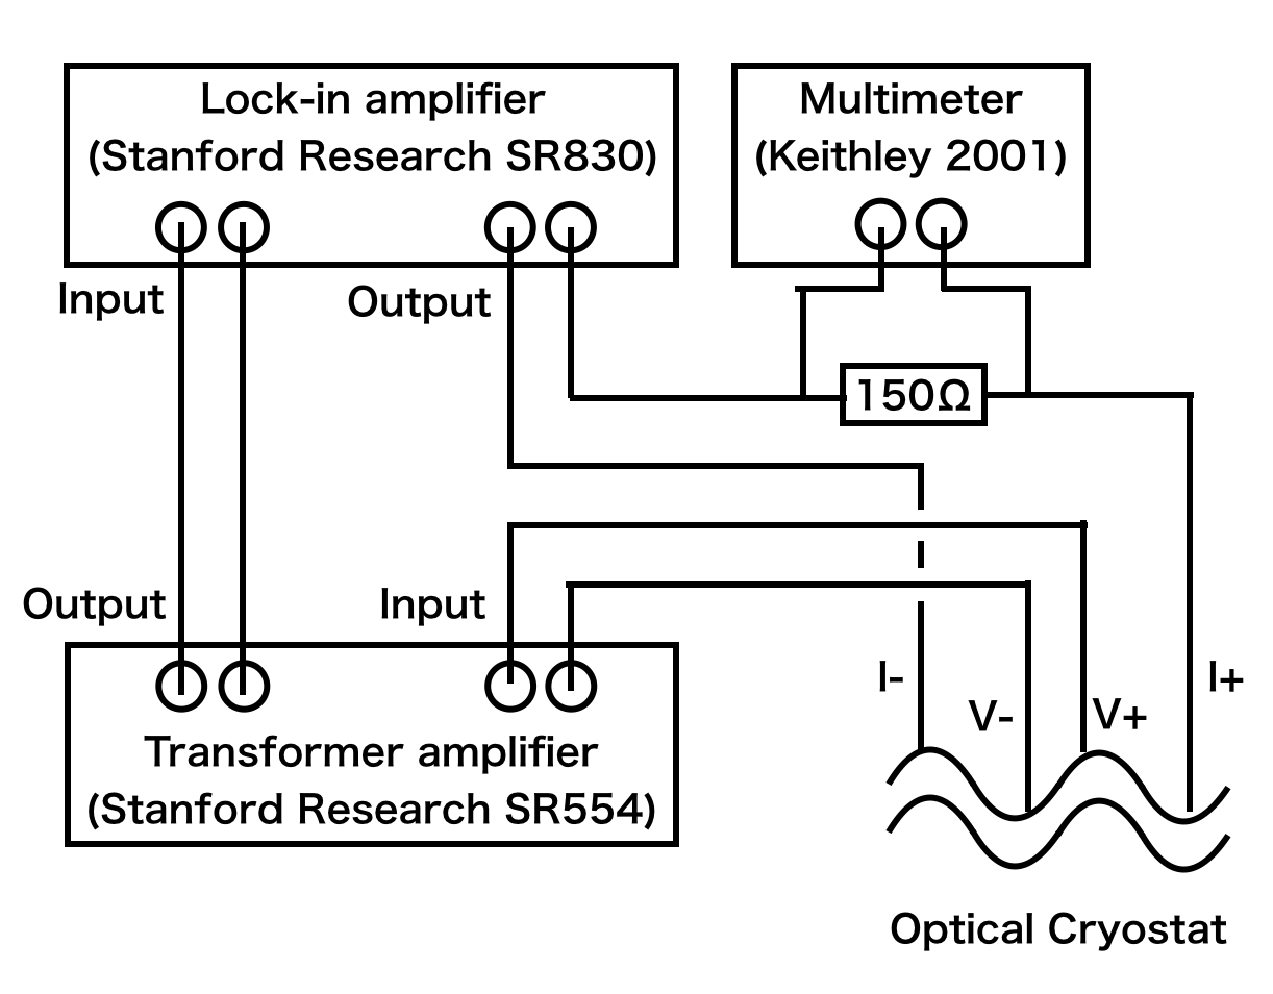
\includegraphics[width=0.7\hsize]{experiment/schematics_lockin.eps}
  \end{center}
  \caption{}
  \label{fig:schematics_lockin}
   \end{minipage}
\end{figure}

\subsection{電流パルスによるα相とβ相の共存状態の生成}
αスズとである。
\begin{figure}[!h]
 \begin{minipage}{\hsize}
    \begin{center}
   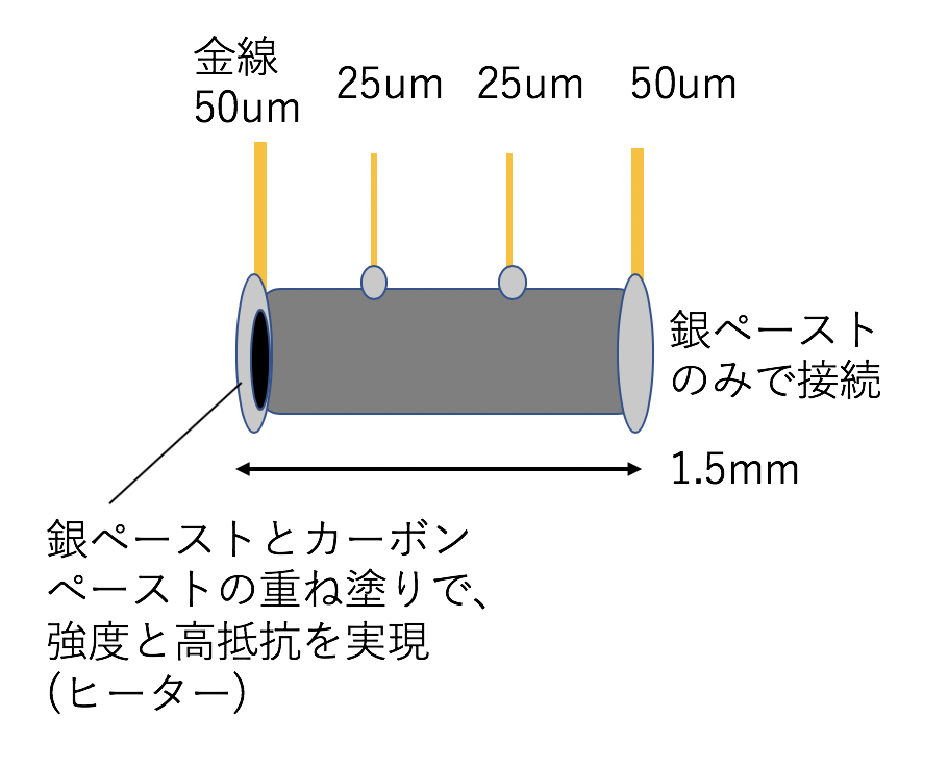
\includegraphics[width=0.7\hsize]{experiment/schematics_sample.eps}
  \end{center}
  \caption{}
  \label{fig:schematics_sample}
 \end{minipage}
 \begin{minipage}{\hsize}
     \begin{center}
   \includegraphics[width=0.9\hsize]{experiment/picture_sample.eps}
  \end{center}
  \caption{}
  \label{fig:picture_sample}
   \end{minipage}
\end{figure}


α相とβ相の共存状態を観察するため、光学顕微鏡を構成した。

%\subsection{電流パルスを用いたβ相からα相への変換}

\clearpage

%\ref{sec:4terminal}